\documentclass[fleqn]{jbook}
\usepackage{physpub}

\begin{document}

\begin{question}{専攻 問題3}{}

% Definition of local macros

\begin{subquestions}
\SubQuestion
  $S$ 座標系と, それに対して $x$-軸方向に速度 $v$ で運動している 
  $S'$ 座標系との間のローレンツ変換は
%
  \begin{eqnarray*}
    ct' &=& +\frac{1}{\sqrt{1 - (v/c)^2}} ct 
            -\frac{v/c}{\sqrt{1 - (v/c)^2}} x \\[-1mm]
    x'  &=& -\frac{v/c}{\sqrt{1 - (v/c)^2}} ct 
            +\frac{1}{\sqrt{1 - (v/c)^2}} x  \\[1mm]
    y'  &=& y \\[2mm]
    z'  &=& z  
  \end{eqnarray*}
%
  である。ただし、二つの座標系は $t=t'=0$ で完全に重なっていたとする。
  $c$ は光の速度である。数学的にはローレンツ変換は世界間隔の $2$乗
%
  \begin{eqnarray*}
     s_{12}^2 = - (ct_2 - ct_1)^2 + (x_2 - x_1)^2%
            + (y_2 - y_1)^2 + (z_2 - z_1)^2
  \end{eqnarray*}
%
  を不変にする座標変換である。次の 3 つの条件からローレンツ変換を導け。

  \begin{itemize}
  \item 世界間隔の 2 乗が不変である。
  \item 座標系の相対性原理 (等速運動している座標系は互いに同等である。)
  \item $v/c \ll 1$ の極限で座標変換はガリレオの座標変換
    \[ t' = t \qquad%
       x' = x - vt \qquad%
       y' = y \qquad%
       z' = z \qquad \]
    に一致する。
  \end{itemize}



\SubQuestion
  光の速さに近い速度 $v$ で走っている電車から振動数 ${\nu}_0$ の光が
  すべての方向に放射されている。電車の進行方向側の線路上に立っている
  観測者が観測する光の振動数 ${\nu}_1$を求めよ。 \\
  また線路と直交している道路の無限遠方で観測したとき光の
  振動数 ${\nu}_2$ はいくらか?


\SubQuestion
  静止状態での長さが $500\Unit{m}$ の電車が光の速さに近い速度で走って
  いる。電車の進行方向に小さな山があり、そのトンネルの長さは
  $400\Unit{m}$である。電車が光の速度の $4/5$ の速さで等速運動しなが
  らこのトンネルを通過することについて以下の問いに答えよ。

  \begin{subsubquestions}
  \SubSubQuestion
    特殊相対論では自分の座標系に対して相対的に速度を持った物体の長さは
    短く観測される。これはローレンツ短縮と呼ばれている。静止時の物体の
    長さ(固有長さ)が $\ell_0$ である物体が観測者の座標系で $x$-軸方向
    に速度$v$で等速運動している。観測者が測定する長さ $\ell$ を求めよ。

  \SubSubQuestion
    電車がトンネルに入り、また出て行くのを近くの丘の上で A 君が観測
    することにした。A 君は、「ローレンツ短縮の効果で、先頭から後尾まで
    電車のすべてが完全にトンネル内に入ってしまい、電車が見えなくなる
    ようなことが起こるはずだ。」と考えた。地面に静止した座標系では
    電車の長さは何 m と推定されるか?

  \SubSubQuestion
    逆に電車に乗っている B 君は、「トンネルこそローレンツ短縮を受けて
    短くなるはずである。したがってどんな時刻においても、電車の先頭、
    後尾の少なくともどちらかはトンネル外にあるはずで、電車の全体が
    トンネル内にあるようなことは起こり得ない。」と考えた。\\
    B 君から見たトンネルの長さはいくらか?

  \SubSubQuestion
    電車の後尾がトンネルに入る時刻を、A 君の時計で、$t_1$ 、
    B 君の時計で、$t_1'$ 、また先頭がトンネルから出てくる時刻を
    A 君の時計で $t_2$ 、B 君の時計で $t_2'$として、
    A 君と B 君の考え方の違いを比較検討し解説せよ。

  \end{subsubquestions}
\end{subquestions}
\end{question}
\begin{answer}{専攻 問題3}{}

\def\xA{x\ssub{A}}
\def\xB{x\ssub{B}}


\begin{subanswers}
\SubAnswer
  時間空間の一様性より変換は1次変換とおける。それゆえ
%
  \begin{eqnarray}
    ct'&=& A\, ct+B\,x \eqname{1}\\
    x'&=& C\,ct+D\,x   \eqname{2}
  \end{eqnarray}
%
  「世界間隔の2乗が不変」より、$-(ct')^2+x^{\prime 2}=-(ct)^2+x^2\quad$であり、
  これに式\eqhref{1},\eqhref{2}を代入して、各係数を比較することにより
%
  \[ A^2-C^2=1 \hspace{10mm} D^2-B^2=1 \hspace{10mm} AB=CD \]
  \begin{equation}
    \Yueni A=D=\cosh \, \theta  \hspace{10mm}  C=B=\sinh \, \theta \eqname{3}
  \end{equation}
%
  とおける。ただし$\theta=\theta (v)$である。$A$と$D$の符号の関係は、
  $\theta$が0のとき$A=D$になることから上のように決まる。
%
  いま、$S'$系が$S$系に対し$x$軸正方向に速度$v$で動いている。このことより、
  $S'$系の$x'=0$の点は$S$系では、$x=vt$であるので、$x$,$t$に依らない定数
  $\gamma=\gamma(v)$を用いて
%
  \begin{equation}
    x'= \gamma (x-vt) \eqname{4}
  \end{equation}
%
  とかける。式\eqhref{3}を式\eqhref{2}に代入して、式\eqhref{4}と
  比較すると
%
  \[ \tanh  \theta = - \frac {v}{c} \]
%
  従って
%
  \begin{equation}
    \cosh \theta = \frac {\pm 1}{\sqrt{1-(v/c)^2}} \hspace{10mm}
    \sinh \theta = \frac {\mp v/c}{\sqrt{1-(v/c)^2}} \eqname{5}
  \end{equation}
%
  $v=0$で\eqhref{1}は$x'=x$になることから式\eqhref{5}の符号は上側になる。
  結局、式\eqhref{1},\eqhref{2}は
%
  \begin{eqnarray*}
    ct'&=& \frac {1}{\sqrt{1-(v/c)^2}} ct-\frac {(v/c)}{\sqrt{1-(v/c)^2}}x \\
     x'&=& -\frac {(v/c)}{\sqrt{1-(v/c)^2}}ct+ \frac {1}{\sqrt{1-(v/c)^2}}x
  \end{eqnarray*}
%
  となり求める変換がえられた。

\SubAnswer
  $S'$系で等方に広がる波
% 
  \begin{equation}
    \psi '= \exp\left[ik'(\sqrt{x^{\prime 2}+y^{\prime 2}+z^{\prime 2}}-ct') \right]  \eqname{6}
  \end{equation}
%
  を考える。但し$k'$は$S'$系から見た波数で、$k'= 2 \pi \nu_0/c$である。\\
%
  光源の前方$x'>0,y'=0,z'=0$で観測すると、$ \psi '= \exp[ik'(x'-ct')]$である。
  これに設問{\bf 1}のローレンツ変換を行うと $S$系では 
%
  \[ \psi=\exp\left[ ik'\frac{1}{\sqrt{1-\beta ^2}}(1+\beta )(x-ct) \right] \]
%
  ただし$\beta = v/c $である。$[ \, ]$の中の$t$の係数は、観測される振動数
  $\nu_1$を用いて$2\pi i\nu_1$である。よって
%
  \[ \nu _1 = \frac {1+\beta }{\sqrt{1-\beta ^2}} \frac{ck'}{2\pi}%
            = \sqrt{\frac{c+v}{c-v}} \nu _0  \]
%
  次に光源が原点を通過するとき、$y$軸上の正の無限遠方で観測する。
  このとき$x=x'=0,\,z=z'=0$であるので$ \psi '= \exp[ik'(y'-ct')]$である。
  これに設問{\bf 1}のローレンツ変換を行うと $S$系では 
%
  \[ \psi = \exp \left[ ik'\left( y-\frac{1}{\sqrt{1-\beta^2}} ct \right) \right] \]
%
  同様に、$tの係数=2\pi i\nu _2 $として
%
  \[ \nu_2 = \frac{1}{\sqrt {1- \beta ^2}} \frac {ck'}{2 \pi}%
           = \frac{1}{\sqrt {1- \beta ^2}} \nu _0 \]
%

\SubAnswer
  \begin{subsubanswers}
  \SubSubAnswer
    棒の両端A、Bを$\xA' =0,\,\xB' =\ell$とする。また、ローレンツ変換より
%
    \begin{eqnarray}
      \xA'&=& - \frac{\beta}{\sqrt{1-\beta ^2}}ct%
              + \frac{1}{\sqrt{1-\beta ^2}} \xA  \eqname{7} \\
      \xB'&=& - \frac{\beta}{\sqrt{1-\beta ^2}}ct%
              + \frac{1}{\sqrt{1-\beta ^2}} \xB  \eqname{8}
    \end{eqnarray}
%
    $S$系からみた棒の長さとは、同じ$t$でみた$\xA$と$\xB$の間隔だから、
    式\eqhref{8}から式\eqhref{7}を引いて
%
    \[ \xB'-\xA'=\frac {1}{\sqrt{1-\beta ^2}} (\xB-\xA) \]
%
    ここで$\xB'-\xA'=\ell$だから、
%
    \[ \xB-\xA=\ell \sqrt{1-\beta ^2} \]
%
  \SubSubAnswer
%
    \[ 500 \times \sqrt{1- \left( \frac {4}{5} \right) ^2}%
       = 500 \times  \frac{3}{5}=300\Unit{[m]} \hspace{5mm}\mbox{答え} \]
%
  \SubSubAnswer
%
    \[ 400 \times \frac{3}{5}=240\Unit{[m]} \hspace{5mm}\mbox{答え} \]
%
  \SubSubAnswer
    ミンコフスキー時空で両者の関係を図示すると下図のようになる。
    図から明らかなように$t_1,t_2$と$t'_1,t'_2$の関係は逆になっている
    ので矛盾はない。

    \begin{center}
      \mbox{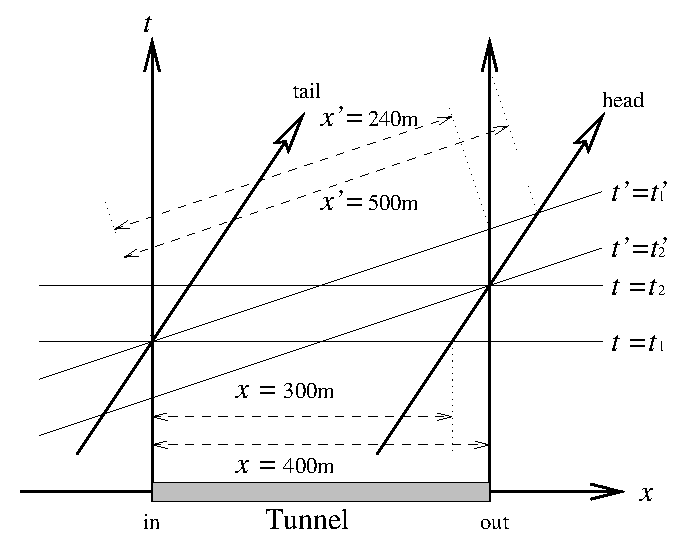
\includegraphics[clip]{1996phy3-1.eps}}
    \end{center}

  \end{subsubanswers}

\end{subanswers}

\end{answer}


\end{document}
